
\documentclass{article}

\usepackage[margin=1in]{geometry}
\linespread{1.2}

\usepackage{amsfonts, amsmath, authblk, graphicx, natbib}

% This nastiness for the bibliography to work both locally and on Overleaf
% https://tex.stackexchange.com/questions/623701/path-for-bib-file-working-simultaneously-in-texstudio-and-overleaf
\bibliographystyle{\ifnum\pdfstrcmp{\jobname}{output}=0 reports/apa-good\else ../apa-good\fi}

\title{Swinging, Fast and Slow:\\Interpreting variation in baseball swing tracking metrics}
\author[1]{Scott Powers}
\author[2]{Ronald Yurko}
\affil[1]{Department of Sport Management, Rice University}
\affil[2]{Department of Statistics \& Data Science, Carnegie Mellon University}

\begin{document}

  \maketitle
	
  \begin{abstract}
    The abstract goes here.
  \end{abstract}

  \section{Introduction}
  \label{sec:introduction}

    Baseball has a long history as fertile ground for statistical analysis of rich datasets. For Major League Baseball (MLB), detailed records are publicly available at the play-by-play level going back to 1912 \citep{retrosheet}. Beginning in 2007, MLB made optical pitch tracking data freely available online
    \citep{fast_what_2010}, enabling unprecedented insights into player performance \citep{swartz_quality_2017}. In 2016, MLB made waves again when they updated their ball tracking technology to incorporate Doppler radar and released batted ball tracking data to the public \citep{arthur_new_2016}. Most recently, in May 2024, MLB released their most exciting new dataset since batted ball tracking 2016: bat tracking at the pitch-by-pitch level \citep{petriello_everything_2024}.

    \begin{figure}
      \centering
      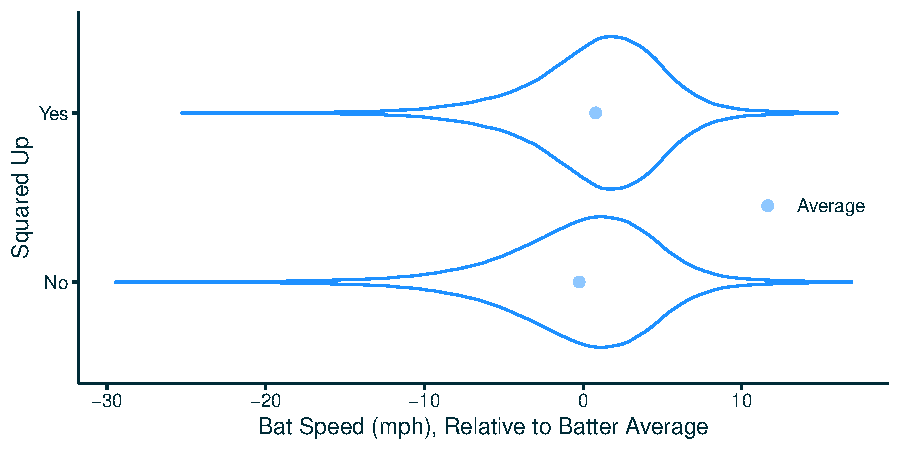
\includegraphics[width = 0.8\textwidth]{../../figures/counterintuitive.pdf}
      \caption{\it Distribution of bat speed relative to batter average by contact quality (squared up or not), across all swings in the dataset. The x-axis represents the difference between the bat speed and the batter's average bat speed. Following MLB's definition, a swing is considered ``squared up'' if the batted ball's exit velocity is at least 80\% of the theoretical maximum (given pitch speed and bat speed), a proxy for good contact.}
      \label{fig:counterintuitive}
    \end{figure}

    \begin{figure}
      \centering
      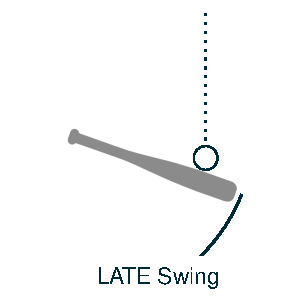
\includegraphics[width = 0.4\textwidth]{../../figures/swing_late.pdf}
      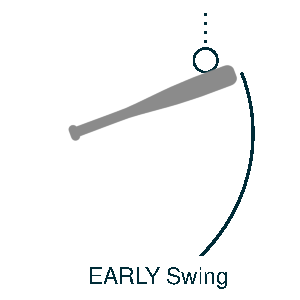
\includegraphics[width = 0.4\textwidth]{../../figures/swing_early.pdf}
      \caption{\it A diagram illustrating the effect of swing timing on swing length measurement due to the fact that swing length is measured at the point of contact. Imagining two swings with the exact same mechanics, the left image shows the swing length measurement if the swing is late, and the right image shows the swing length measurement if the swing is early.}
      \label{fig:swing-diagram}
    \end{figure}

    \subsection{Related Work}
    \label{sec:related-work}

      \begin{itemize}
        \item Bat tracking
        \begin{itemize}
          \item \citet{nevins_sensitivity_2019}
          \item \citet{orishimo_lower_2024}
          \item \citet{nakashima_acceptable_2025}
        \end{itemize}
        \item Bat tracking (blogs)
        % Candidates
        % https://blogs.fangraphs.com/what-statcasts-new-bat-tracking-data-does-and-doesnt-tell-us/
        % https://blogs.fangraphs.com/daddy-hacks-or-the-lone-peril-of-swinging-too-hard/
        % https://www.baseballprospectus.com/news/article/95688/best-of-bp-in-defense-of-isaac-paredes/
        % https://www.drivelinebaseball.com/2024/07/using-mlb-bat-tracking-data-to-better-understand-swings/
        % https://theadvancescout.substack.com/p/whats-in-a-swing-a-metrics-explainer
        % https://theadvancescout.substack.com/p/the-radar-gun-doesnt-work-here
        % https://theadvancescout.substack.com/p/the-cheat-swing
        \begin{itemize}
            \item 
        \end{itemize}
        \item Skew normal
        \begin{itemize}
          \item \citet{judge_exit_2024}
        \end{itemize}
        \item Instrumental variable regression
        \begin{itemize}
          \item \citet{putman_tackling_2025}
        \end{itemize}
      \end{itemize}

  \section{Data}
  \label{sec:data}

    Our dataset comprises 685,143 pitches thrown during the 2024 MLB regular season. This publicly available dataset was downloaded from Baseball Savant \citep{baseball_savant} using the R package sabRmetrics \citep{sabRmetrics}. For each pitch, we observe the identities and handedness (left/right) of the batter and pitcher involved and the ball-strike count prior to the pitch. We also observe pitch tracking information, most notably the pitch type (e.g. fastball, curveball, changeup) and the $(x, z)$ location where the pitch crosses the front of home plate. The pitch tracking information is sufficient to recreate an estimate of the pitch's full trajectory as a three-dimensional quadratic function of time $(x(t), y(t), z(t))$ and to recreate the corresponding pitch metrics such as release point, release speed, and vertical/horizontal break. Each pitch has a categorical outcome, which can be one of: hit by pitch, called ball, called strike, swinging strike, foul ball, or hit into play.

    For pitches on which the batter swings, we observe bat tracking information describing the bat speed and the swing length (detailed in Section \ref{sec:measurement}). For pitches that are hit into play, we observe the initial exit speed and vertical exit angle (relative to the ground) of the ball as it leaves the bat. We also observe each fair batted ball's manually charted hit coordinates (on the field), which serves as a proxy for the horizontal exit angle of the ball off the bat.

    \subsection{Bat Speed and Swing Length Measurement}
    \label{sec:measurement}

      Bat tracking metrics were made possible by improvements to MLB's Hawk-Eye Statcast system in 2023 which featured five high frame rate (300 frames per second) cameras dedicated to tracking movements of the pitcher and the batter \citep{goldbeck_introducing_2023}. Through computer vision, this system tracks not only player center of mass but full limb orientation (including the bat) throughout the pitching and batting movements, generating a rich kinematic time series of data on each pitch.

      The raw kinematic time series data are not publicly available, but MLB has begun to release some metrics derived from them, starting with bat speed and swing length on every pitch. Bat speed is defined as the linear speed of the ``sweet spot'' of the bat (roughly six inches from the end) at the point of contact with the ball, and swing length is defined as the distance travelled by the end of the bat from the start of the swing until the point of contact \citep{petriello_everything_2024}. In the event of a swing and miss, both metrics are measured at the point nearest to contact. These metrics represent a tiny fraction of the kinematic time series data, and the process by which they are measured complicates their interpretation on a swing-by-swing basis.

    \subsection{Data Cleaning}

  \section{Methods}
  \label{sec:methods}

    \subsection{Intention Model}
    \label{sec:methods-intention}

    We begin with the hypothesis that two covariates explain real (non-artifactual) differences in swing mechanics: ball-strike count and pitch location. To the extent that a batter’s swing tracking metrics co-vary with count, we describe this as their \textit{approach}. To the extent that a batter’s swing tracking metrics co-vary with pitch location, we describe this as swing \textit{adaptation}. Acknowledging that swing timing biases the measurement of bat speed and swing length, we mitigate this confounding bias by filtering on swings that result in squared-up contact against pitchers' primary fastballs. Additionally, based on visualizations of batter swing length and bat speed distributions (such as examples in INSERT FIGURE REFERENCE?) we are also interested in capturing variation in the shape of the intended distributions for hitters. 

    To this end, we fit the following skew-normal (SK) multilevel model:

    \begin{align}
    \label{eqn:intention-swing-length}
    \begin{split}
        ( \mbox{swing length} )_i &\sim \mbox{SK}(\mu_i, \sigma, \alpha_i) \\
        \mu_i &= \mu_0 + \gamma_{p_i} + \gamma_{b_i}
        + \beta^B \cdot (\mbox{balls})_i
          + (\beta^S + \gamma^S_{b_i}) \cdot (\mbox{strikes})_i\\
        & + (\beta^X + \gamma^X_{b_i}) \cdot (\mbox{pitch loc x})_i
          + (\beta^Z + \gamma^Z_{b_i}) \cdot (\mbox{pitch loc z})_i \\
          \alpha_i &= \alpha_0 + \nu_{b_i}
    \end{split}
    \end{align}
    where $b_i$ denotes the batter on swing $i$ against pitcher $p_i$. We use the same specification for both swing length and bat speed intention models. 
    
    In detail, the $\gamma$ parameters are random intercepts and random slopes describing the mean of the swing distribution such that,

    \begin{align}
        \begin{split}
            \gamma_{p_i} &\sim \mathcal{N}(0, \sigma^2_p) \\
            \boldsymbol{\gamma}_{b_i} &\sim \mathcal{N}(\boldsymbol{0}, \Sigma)
        \end{split}
    \end{align}
    where $\boldsymbol{\gamma}_{b_i}$ is the vector of batter random intercept and slopes $(\gamma_{b_i}, \gamma^S_{b_i}, \gamma^X_{b_i}, \gamma^Z_{b_i})$ which follow a multivariate normal distribution centered around the zero vector $\boldsymbol{0}$ with covariance matrix $\Sigma$. This $\Sigma$ contains the relevant random effect variances for the batter-level terms, $(\sigma_b, \sigma_b^S, \sigma_b^X, \sigma_b^Z)$, as well as their respective correlations. This allows us to quantify variation between hitters and pitchers at the intercept level, as well as capture variation in batter approach and swing adaptation.
    
    The $\nu_{b_i}$ parameters are random intercepts enabling us to capture variation between batters in the shape $\alpha$ of the swing length and bat speed distributions, where
    \begin{equation}
        \nu_{b_i} \sim \mathcal{N}(0, \tau^2_b).
    \end{equation}

    These models tell us: What are the bat speed and swing length (by batter, count and pitch location) when the timing is good? We interpret the prediction from this model on each pitch as the intended bat speed and swing length.
    
    We fit both bat speed and swing length models in a Bayesian framework via the brms package in R \citep{brms}, which provides an interface for Bayesian modeling with Stan \citep{carpenter2017stan}. We use weakly informative priors for the parameters, with vague half-$t_3$ priors (i.e., a Student's $t$ distribution centered at zero with 3 degrees of freedom but truncated to positive values) for the standard deviation parameters \citep{gelman2006prior} and the LKJ prior for the correlations between batter-level effects \cite{lewandowski2009generating}. Our Bayesian approach naturally provides uncertainty quantification for the model parameters via their posterior distributions, which are estimated using MCMC sampling. For model fitting, we use four parallel chains with 6,000 (3,000 burn-in) and 4,000 (2,000 burn-in) samples for the swing length and bat speed models respectively. We observe evidence of convergence of the MCMC algorithm based on observing trace plots and $\hat{R}$ statistics close to 1 \citep{gelman1992inference, brooks1998general}, along with no indication of problematic effective sample sizes \citep{gelman2020bayesian}. 
    
    For comparison, we also fit simpler Gaussian versions of the swing length and bat speed models. These models follow a specification similar to that of the SK models in Equation \ref{eqn:intention-swing-length}, but with the shape parameter removed (i.e., the Guassian distribution is a SK with shape equal to 0). We use an 80/20 train/test split to compare the out-of-sample performance of the SK and Gaussian fits against each other. We compute the expected log pointwise predictive density (ELPD) on the 20\% test data, which involves computing the log-likelihood of each test observation for each posterior sample. In addition to providing us with standard errors about the difference in model performance, we choose ELPD as our evaluation metric because of our interest in comparing the skewness of the SK posterior predictive distributions relative to the symmetric Gaussian.

    \subsection{Causal Model}
    \label{sec:methods-causal}

      The intention model from Section \ref{sec:methods-intention} sets us up to estimate a causal model for the effect of bat speed and swing length on swing outcomes via instrumental variables regression (CITATION). Relying on baseball domain knowledge, we hypothesize that the relationship between swing tracking metrics and outcomes is confounded by a latent, unobserved variable: whether the batter correctly identifies the pitch type early in its trajectory (by lucky guess or by other means) or needs to make a mid-swing adjustment. When the batter fails to correctly identify the pitch type early, he is less likely to make good contact, and he also adjusts his swing, reducing the bat speed and affecting the swing length. Critically, this confounder can vary significantly from pitch to pitch as batters frequently limit their focus to one or two pitch types because it is too difficult to prepare for any pitch type (CITATION).

      A good instrumental variable is one which has an effect on the treatment (in this case, swing tracking metrics) and is known to be uncorrelated with the confounder (CITATION). As the instrument varies, we observe the effect of the treatment with the effect of the confounder stripped away. Relying on the framework from Section \ref{sec:methods-intention}, we choose the batter's count-intended bat speed and swing length as our instrumental variables. Count-intended swing length is the player specific contribution of count to swing length, as estimated by (\ref{eqn:intention-swing-length}), and count-intended swing length is defined analogously.

      Count-intended swing metrics affect observed swing metrics as modeled in Section \ref{sec:methods-intention}, and we expect that they are approximately uncorrelated with early pitch recognition. The count is known before the pitch and does not depend on the pitch itself. This may not be a perfect instruction, for example, if batters who tend to struggle more with early pitch recognition in two-strike counts tend also to modify their two-strike swing intentions a certain way. But this choice of instrumental variables will mitigate any confounding effect of early pitch recognition from pitch to pitch.

      We consider the effect of bat speed and swing length on three components of the pitch outcome model: probability of contact conditioned on swing; probability of fair ball conditioned on contact; and expected xwOBA conditioned on fair ball. For each of these components, we estimate a logistic or linear regression of the outcome on the batter's count-intended bat speed and swing length, with an offset for the prediction from the pitch outcome model described in Section \ref{sec:methods-pitch-outcome-model}. This offset controls for the difficulty of each pitch when estimating the effects of count-based bat speed and swing length adjustments.

      Using $i \in \{1, ..., n\}$ to index swings, the random variables $Y_i^{\mbox{\scriptsize con}} \in \{0, 1\}$, $Y_i^{\mbox{\scriptsize fair}} \in \{0, 1\}$ and $Y_i^{\mbox{\scriptsize xwOBA}} \in \mathbb{R}$ represent whether swing $i$ results in contact; whether swing $i$ results in a fair ball; and the xwOBA of the batter ball on swing $i$ (undefined if $Y_i^{\mbox{\scriptsize fair}} \in \{0, 1\} = 0$), respectively. The corresponding predictions from the pitch outcome model are denoted by $\hat p_i^{\mbox{\scriptsize con}} \in (0, 1)$,  $\hat p_i^{\mbox{\scriptsize fair}} \in (0, 1)$ and $\hat y_i^{\mbox{\scriptsize xwOBA}} \in \mathbb{R}$. We use $b_i$ to denote the batter on swing $i$, and $\hat\gamma_{b_i}^{\mbox{\scriptsize BS}}$ and $\hat\gamma_{b_i}^{\mbox{\scriptsize SL}}$ are the estimated batter random slopes for strikes in the bat speed intention model and the swing length intention model, respectively.

      \begin{align}
        \label{eqn:causal-contact}
        \log \left(
          \frac{\mathbb{P}(Y_i^{\mbox{\scriptsize con}} = 1)}{1 - \mathbb{P}(Y_i^{\mbox{\scriptsize con}} = 1)}
        \right) &= \log \left(
          \frac{\hat p_i^{\mbox{\scriptsize con}}}{1 - \hat p_i^{\mbox{\scriptsize con}}}
        \right) +
          \alpha^{\mbox{\scriptsize con}} +
          \beta_{\mbox{\scriptsize BS}}^{\mbox{\scriptsize con}} \cdot
            \hat\gamma_{b_i}^{\mbox{\scriptsize BS}} +
          \beta_{\mbox{\scriptsize SL}}^{\mbox{\scriptsize con}} \cdot
            \hat\gamma_{b_i}^{\mbox{\scriptsize SL}},\\[10pt]
        \label{eqn:causal-fair}
        \log \left(
          \frac{
            \mathbb{P}(Y_i^{\mbox{\scriptsize fair}} = 1 \mid Y_i^{\mbox{\scriptsize con}} = 1)
          }{
            1 - \mathbb{P}(Y_i^{\mbox{\scriptsize fair}} = 1 \mid Y_i^{\mbox{\scriptsize con}} = 1)
          }
        \right) &= \log \left(
          \frac{\hat p_i^{\mbox{\scriptsize fair}}}{1 - \hat p_i^{\mbox{\scriptsize fair}}}
        \right) +
          \alpha^{\mbox{\scriptsize fair}} +
          \beta_{\mbox{\scriptsize BS}}^{\mbox{\scriptsize fair}} \cdot
            \hat\gamma_{b_i}^{\mbox{\scriptsize BS}} +
          \beta_{\mbox{\scriptsize SL}}^{\mbox{\scriptsize fair}} \cdot
            \hat\gamma_{b_i}^{\mbox{\scriptsize SL}},\\[10pt]
        \label{eqn:causal-hit}
        Y_i^{\mbox{\scriptsize xwOBA}} \mid \{Y_i^{\mbox{\scriptsize fair}} = 1\} &\sim
          \mbox{Normal}\left(
            \hat y_i^{\mbox{\scriptsize xwOBA}} +
              \alpha^{\mbox{\scriptsize xwOBA}} +
              \beta_{\mbox{\scriptsize BS}}^{\mbox{\scriptsize xwOBA}} \cdot
                \hat\gamma_{b_i}^{\mbox{\scriptsize BS}} +
              \beta_{\mbox{\scriptsize SL}}^{\mbox{\scriptsize xwOBA}} \cdot
                \hat\gamma_{b_i}^{\mbox{\scriptsize SL}},
            \sigma^2
          \right).
      \end{align}

      In each of these models, we interpret $\alpha^\cdot$ as an intercept to account for the fact that the mean outcome may not be the same in this dataset as in the dataset on which the pitch outcome model was trained. We interpret $\beta_{\mbox{\scriptsize BS}}^{\cdot}$ and $\beta_{\mbox{\scriptsize SL}}^{\cdot}$ as the effects of bat speed and swing length adjusments on the outcomes. The parameter $\sigma^2$ in the xwOBA model is a nuisance parameter.

    \subsection{Run Value Model}
    \label{sec:methods-value}

      The models from Section \ref{sec:methods-causal} estimate the effect of swing adjustments on contact and power, but they don't dhelp us make value judgments when these effects move in opposite directions, e.g. sacrificing power for increased contact. In baseball, the units of value are runs, which translate directly to wins (CITATION). The standard metric for estimating the run value of batting performance is linear weight, which assigns a run value to each type of batter outcome (strikeout, walk, home run, etc.) according to its average change in base-out run expectancy (CITATION). In this section, we describe a method for converting the effects on contact and power into effects on linear weight.

  \section{Results}
  \label{sec:results}
  

    \subsection{Intention Model}
    \label{sec:results-intention}

    The out-of-sample ELPD results are shown in Table \ref{tab:intention-model-elpd} for both swing length and bat speed models. For both settings, the SK model displayed an ELPD of around 3 standard errors better than the Gaussian model. The remaining results in this manuscript are based on the SK intention models.

\begin{table}
        \centering
        \begin{tabular}{l|r|r|r|}
          & $\Delta$ELPD  & SE & \# SEs \\
          \hline
          Swing length & 34.1279 & 11.7237 & 2.9110 \\ 
  Bat speed & 87.6000 & 27.8787 & 3.1422 
        \end{tabular}
        \caption{\it Model comparison via expected log predictive density (ELPD). Shown are the difference in EPLD between the skew-normal (SK) and Gaussian models ($\Delta$ELPD), the standard error of ELPD difference (SE), and the number of standards errors the SK model is better than the Gaussian model.}
        \label{tab:intention-model-elpd}
      \end{table}

       Table \ref{tab:fixed-effects} summarizes the fixed effects of the bat speed and swing length intention models. We observe intuitive relationships for both models with regards to the relationships between pitch-level context and each observed swing measurement. As the number of balls increase, on average ($\beta^B$) we observe faster and longer swings. The opposite behavior is observed as the number of strikes increases ($\beta^S$), with slower and shorter swings on average. Figure \ref{fig:approach} displays the joint distribution of the posterior mean for the batter random slopes for strikes ($\hat{B}^S + \hat{\gamma}_b^S$) in both intention models, regardless of the individual batter effect we expect a decrease in bat speed and swing length per strike. A similar relationship is observed for pitches with higher vertical locations ($\beta^Z$). The two models diverge with regards to the horizontal location of pitches ($\beta^X$), as pitches that thrown further away from the batter result in longer but slower swings on average. With regards to the shape parameter of the SK distribution, the intercepts ($\alpha_0$) for both bat speed and swing length are negative which indicate left skewed distributions.

      \begin{figure}
        \centering
        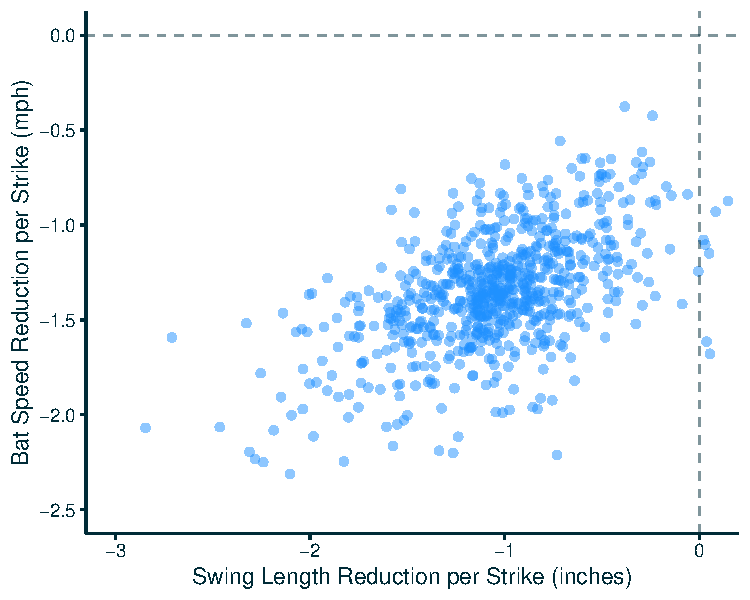
\includegraphics[width = 0.6\textwidth]{../../figures/approach.pdf}
        \caption{\it Estimated batter random slopes for strikes in the intention model. Each point is a batter $b$, with the x-value representing $\hat\beta^S + \hat\gamma^S_b$ from the model (\ref{eqn:intention-swing-length}) and the y-value representing the same quantity from the model (\ref{eqn:intention-bat-speed}). This quantity is interpretable as the expected change in swing length (or bat speed) corresponding to a one-strike increase in the ball-strike count.}
        \label{fig:approach}
      \end{figure}

      \begin{table}
        \centering
        \begin{tabular}{l|rrr|rrr|}
                  & \multicolumn{3}{c|}{Bat Speed}          & \multicolumn{3}{c|}{Swing Length}  \\
        Parameter & Mean  & Lower  & Upper & Mean  & Lower  & Upper \\
          \hline
          \begin{tabular}{l|rrr|rrr|}
    & \multicolumn{3}{c|}{Bat Speed}          & \multicolumn{3}{c|}{Swing Length}  \\
  Parameter & Mean  & Lower  & Upper & Mean  & Lower  & Upper \\
  \hline
  $\mu_0$ & 76.43 & 76.06 & 76.80 & 8.25 & 8.20 & 8.29 \\
  $\beta^B$ & 0.55 & 0.51 & 0.59 & 0.05 & 0.04 & 0.05 \\
  $\beta^S$ & --1.13 & --1.20 & --1.06 & --0.14 & --0.14 & --0.13 \\
  $\beta^X$ & --0.52 & --0.66 & --0.39 & 0.16 & 0.14 & 0.17 \\
  $\beta^Z$ & --1.87 & --2.00 & --1.75 & --0.46 & --0.47 & --0.44 \\
  $\alpha_0$ & --1.85 & --1.96 & --1.75 & --1.46 & --1.56 & --1.36 \\
\end{tabular}
        \end{tabular}
        \caption{\it Posterior mean and 95\% credible interval lower/upper bounds for the fixed effects in the bat speed and swing length intention models.}
        \label{tab:fixed-effects}
      \end{table}

      Next, Table \ref{tab:intention-variances} summarizes the posterior distributions of the random effects variance terms. For both bat speed and swing length intention models, we observe the highest variation is attributed to differences between batters ($\sigma_b$). Interestingly, the variation between batters in the shape random effects ($\tau_b$) is the second highest for swing length but is smaller than the pitch location random slopes ($\sigma_b^X$ and $\sigma_b^Z$) for the bat speed model. For each of the estimated terms, all of the 95\% credible intervals are strictly greater than zero demonstrating evidence of variability between batters at the intercept and slope-level.
       
      \begin{table}
        \centering
        \begin{tabular}{l|rrr|rrr|}
                  & \multicolumn{3}{c|}{Bat Speed}          & \multicolumn{3}{c|}{Swing Length}  \\
        Parameter & Mean  & Lower  & Upper & Mean  & Lower  & Upper \\
          \hline
          $\sigma_p$ & 0.47 & 0.41 & 0.53 & 0.12 & 0.11 & 0.13 \\
$\sigma_b$ & 3.35 & 3.04 & 3.67 & 0.43 & 0.40 & 0.47 \\
$\sigma_b^S$ & 0.42 & 0.35 & 0.50 & 0.05 & 0.05 & 0.06 \\
$\sigma_b^X$ & 1.04 & 0.90 & 1.18 & 0.11 & 0.10 & 0.13 \\
$\sigma_b^Z$ & 1.05 & 0.94 & 1.17 & 0.13 & 0.11 & 0.14 \\
$\tau_b$ & 0.67 & 0.52 & 0.85 & 0.34 & 0.08 & 0.57 \\

        \end{tabular}
        \caption{\it Posterior mean and 95\% credible interval lower/upper bounds for the standard deviation of the random effect terms in the bat speed and swing length intention models.}
        \label{tab:intention-variances}
      \end{table}

      Figure \ref{fig:intent-re} provides an overview of the batter-level $\mu_i$ random effects in the SK intention models. The variation we observe between batters aligns with intuition, as batters known for taking longer/faster swings (e.g., Oneil Cruz, Giancarlo Stanton, Javier Baez) display higher random intercepts ($\gamma_b$) in compare to batters with shorter/slower swings (e.g., Luis Arraez). We observe positive correlations between the random slopes of bat speed and swing length, providing information on the variation between batters with respect to their approach ($\gamma_b^S$) and adaptation ($\gamma_b^X$, $\gamma_b^Z$). For example, Anthony Rizzo's approach appears to be more conservative with the biggest decrease in bat speed and swing length for each additional strike relative to the average batter slope. We also observe batters that deviate from the consistent pattern between bat speed and swing length, such as Shohei Ohtani with regards to his horizontal pitch location random slope appearing to be higher than average for swing length despite a lower than average value for bat speed. 
      
      \begin{figure}
        \centering
        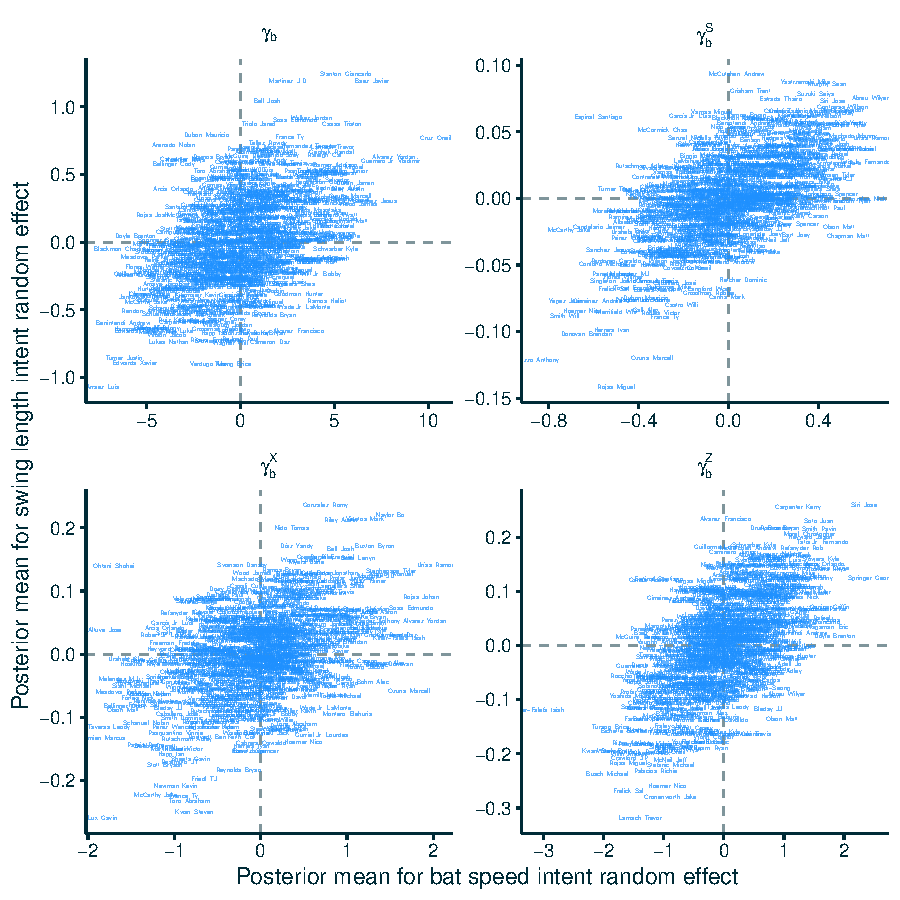
\includegraphics[width = 0.8\textwidth]{../../figures/intent_re.pdf}
        \caption{\it Joint distribution of the posterior means for the batter-level $\mu_i$ random effects in the SK intention models for both bat speed and swing length. Each batter is displayed by their name, and only batters with at least 25 squared-up swings are displayed.}
        \label{fig:intent-re}
      \end{figure}
        
       In contrast, Figure \ref{fig:alpha-re} displays the joint distribution of the posterior means for the batter random intercepts in modeling the shape parameter $\alpha$ of the SK distribution. Unlike the mean-level random effects, we do not observe correlation between the bat speed and swing length shape-level random intercepts. The variation captured by these random intercepts provides some understanding of the differences in the intended swing distribution for players. Luis Arraez displays above average random intercepts for both bat speed and swing length, indicating that his intention distributions are less skewed left than compared to other batters. 
                
      \begin{figure}
        \centering
        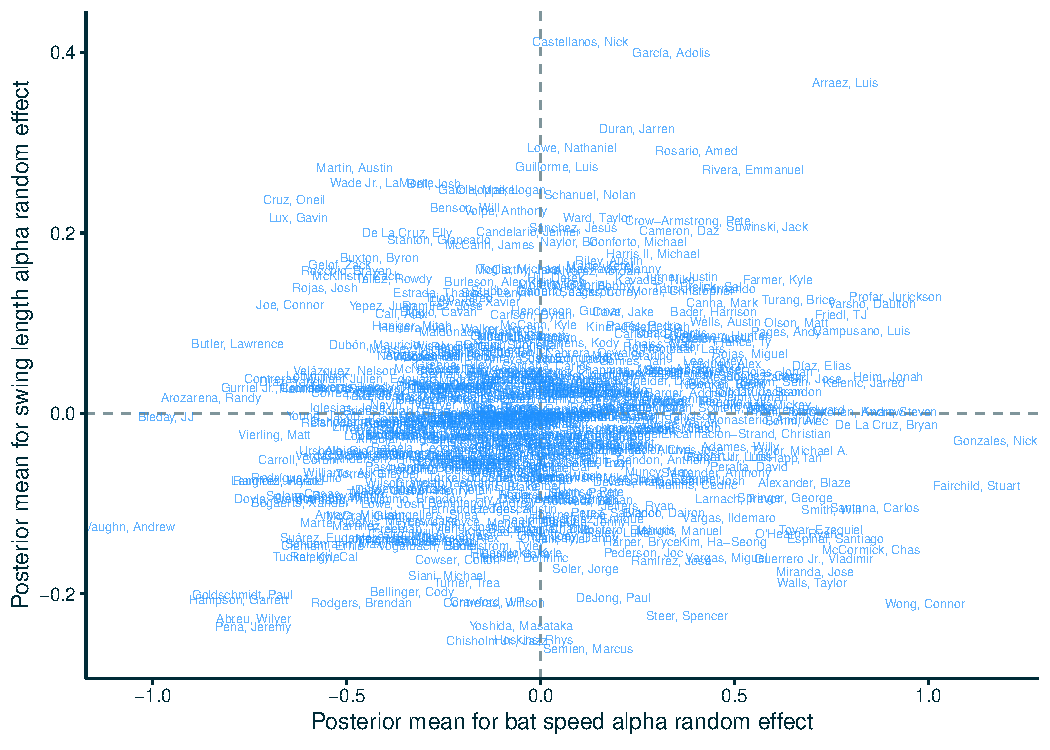
\includegraphics[width = 0.8\textwidth]{../../figures/alpha_re.pdf}
        \caption{\it Joint distribution of the posterior means for the batter-level $\alpha_i$ random effects in the SK intention models for both bat speed and swing length. Each batter is displayed by their name, and only batters with at least 25 squared-up swings are displayed.}
        \label{fig:alpha-re}
      \end{figure}
      
    \subsection{Causal Model}
    \label{sec:results-causal}

      The previous section demonstrates that there are differences between batters in how they modulate their swing length and bat speed as the number of strikes in the count increases. This section addresses the consequences of those differences between batters. As described in Section \ref{sec:methods-causal}, we estimate three separate regression models with instrumental variables for contact probability given swing (\ref{eqn:causal-model-contact}), fair ball probability given contact (\ref{eqn:causal-model-fair}) and expected xwOBAcon given fair ball (\ref{eqn:causal-model-hit}). The estimated effects of bat speed appraoch and swing length approach from these models are reported in Table \ref{tab:causal-model}.

      \begin{table}
        \centering
        \begin{tabular}{l|r|r|r|}
          & Contact Model (\ref{eqn:causal-contact}) & Fair/Foul Model (\ref{eqn:causal-fair}) & xwOBAcon Model (\ref{eqn:causal-hit})\\
          \hline
          \begin{tabular}{l|r|r|r|}
    & Contact Model (\ref{eqn:causal-contact}) & Fair/Foul Model (\ref{eqn:causal-fair}) & xLW Model (\ref{eqn:causal-hit})\\
  \hline
  Bat Speed Approach (mph) & $-0.177 \pm0.016$ & $-0.075 \pm0.014$ & $0.023 \pm0.004$ \\ 
  Swing Length Approach (inches) & $-0.050 \pm0.010$ & $0.003 \pm0.009$ & $0.000 \pm0.002$ 
\end{tabular}
        \end{tabular}
        \caption{\it Estimated regression coefficients and corresponding standard errors from the causal models (\ref{eqn:causal-contact})--(\ref{eqn:causal-hit}). Bat Speed Approach is defined as the batter's change in bat speed per strike added to the count, as estimated by (\ref{eqn:intention-bat-speed}). Swing Length Approach is defined analogously as the batter's change in swing length per strike added to the count, as estimated by (\ref{eqn:intention-swing-length}).}
        \label{tab:causal-model}
      \end{table}

      From the contact model, the negative coefficient $-0.177$ for bat speed approach shows that batters who reduce their bat speed more per strike (i.e. more negative bat speed approach) make contact more often in 1-strike and 2-strike counts. Similarly, the negative coefficient for swing length approach shows that batters who reduce their swing length more per strike make contact more often in these counts. These results match our intuition from baseball domain knowledge: More conservative swings are more likely to make contact, a more plausible conclusion than the counterintuitive results from the naive analysis shown in Figure \ref{fig:counterintuitive}. Bat speed approach and swing length approach have similar between-batter variance, so in comparing the coefficients we observed that bat speed approach has a much greater effect (more than 3x) on contact than does swing length approach. The fair ball probability model shows a similar effect direction for bat speed approach and no effect for swing length approach.

      From the xwOBAcon model (i.e. the ``power'' model), the positive coefficient $0.023$ for bat speed approach shows that batters who reduce their bat speed more per strike (i.e. more negative bat speed approach) exhibit less power in 1-strike and 2-strike counts when they do make contact. This demonstrates evidence for the intuitive tradeoff involved when taking more conservative swings when facing more strikes: greater contact but less power. Swing length approach does not seem to have an effect on power.

      \begin{figure}
        \centering
        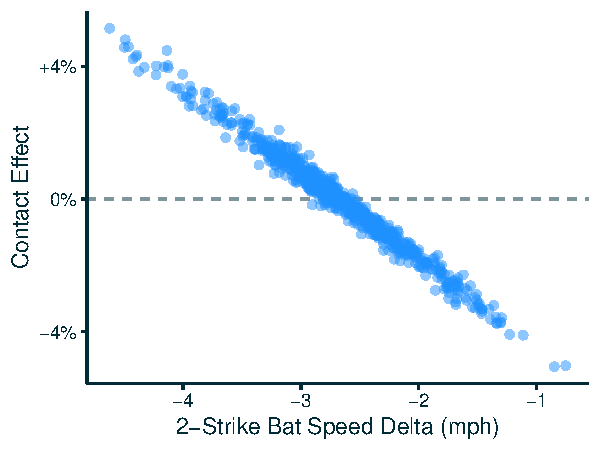
\includegraphics[width = 0.49\textwidth]{../../figures/bat_speed_contact.pdf}
        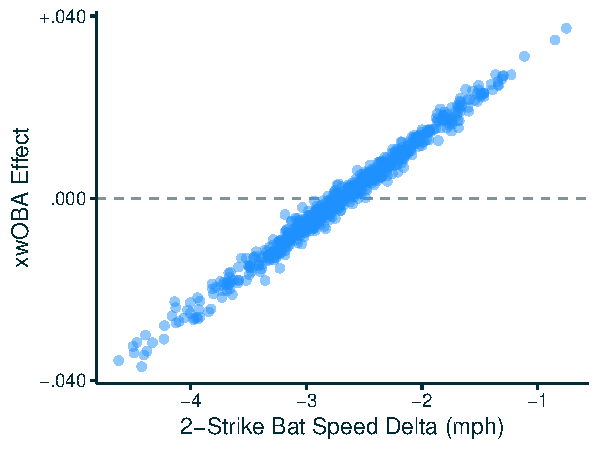
\includegraphics[width = 0.49\textwidth]{../../figures/bat_speed_power.pdf}
        \caption{\it Estimated causal effect of bat speed on contact (left) and power (right). Each point is a batter; the x-axis shows how much the batter slows their swing in two-strike counts, relative to zero-strike counts, from the model (\ref{eqn:intention-bat-speed}); the y-axis shows the estimated combined effect of the batter's bat speed and swing length adjustments on contact rate (left) and xwOBAcon (right) in two-strike counts, from the model (\ref{eqn:causal}). Contact rate is the percentage of swings contacting the ball, and xwOBAcon is a standard sabermetric statistic for measuring power. Its units are runs per plate appearance.}
        \label{fig:results-causal}
      \end{figure}

      The magnitudes of the coefficients in Table \ref{tab:causal-model} are difficult to interpret because two of the models are logistic regressions, so the coefficients represent additive effects in the log-odds scale. For example, a pitch with almost 0\% contact probability will still have almost 0\% contact probability, regardless of approach. The effect of approach on contact is maximized for pitches near 50\% contact probability. Figure \ref{fig:approach} conveys the average effect size across all 2-strike pitches. We observe that the approach effects for almost all batters (relative to an average approach) are within $\pm4\%$ contact probability and $\pm.040$ xwOBA, i.e. $\pm 40$ points of xwOBA.

    \subsection{Run Value Model}
    \label{sec:results-value}

      The previous section demonstrates that there is a contact/power tradeoff involved when batters modulate their swing length and bat speed as the number of strikes in the count increases. This section addresses whether the tradeoff is worthwhile. As described in Section \ref{sec:methods-value}, we estimate the expected linear weight of plate appearance outcomes for the average batter if they were to adopt different approaches. Figure \ref{fig:approach-run-value} plots batter approaches (as previously plotted in Figure \ref{fig:approach}) now with a color gradient in the background showing the estimated run value of each approach.

      \begin{figure}
        \centering
        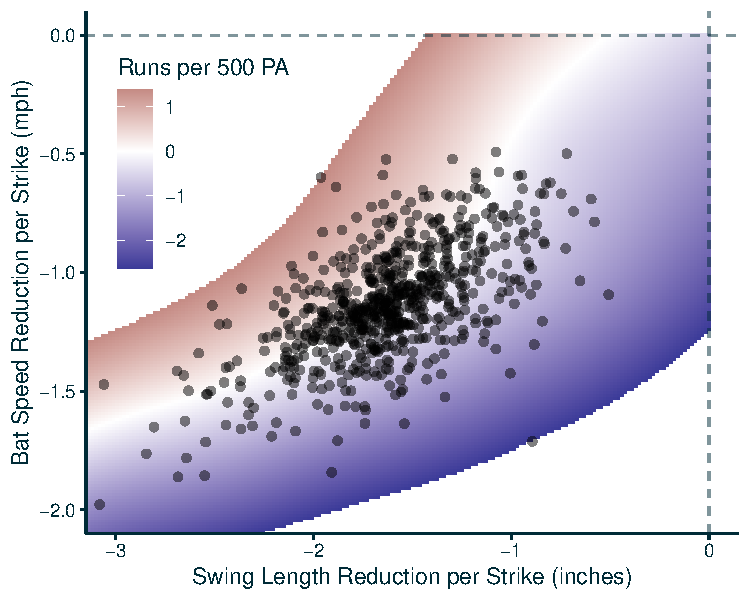
\includegraphics[width = 0.8\textwidth]{../../figures/approach_run_value.pdf}
        \caption{\it Estimated causal effect of batters' approaches, measured on the scale of runs per 500 plate appearances (PA). This figure shows the same data as Figure \ref{fig:approach} except that the background gradient reports the estimated run value of each approach. If an approach is valued at z runs, the interpretation is that the average batter with this approach is expected to produce z runs more than if they adopted an average approach, as measured by linear weights.}
        \label{fig:approach-run-value}
      \end{figure}

      The magnitude of the difference between the higest-value approaches and the lowest-value approaches is small, approximately 4 runs per 500 plate appearances. To put this in context, it amounts to a difference of roughly half a win per season[CITATION]. Baseball teams are chasing increasingly small competitive advantages[CITATION], and the cost of half a win is roughly \$5 million in the free agent market[CITATION]. We observe that the highest-value approaches are those which cut down on swing length without cutting down on bat speed. From Table \ref{tab:causal-model}, we can see that this is a way to avoid the contact/power tradeoff because cutting down on swing length (all else equal) increases contact without decreasing power.

      \begin{table}
        \centering
        \begin{tabular}{rl|rr|r}
          &        & \multicolumn{2}{c|}{Approach}          & Runs /\\
          & Batter & Bat Speed (mph)  & Swing Length (in.)  & 500 PA\\
          \hline
          \begin{tabular}{rl|rr|r}
& & \multicolumn{2}{c|}{Approach} & Runs /\\
 & Batter & Bat Speed (mph) & Swing Length (in.) & 500 PA \\
% latex table generated in R 4.5.0 by xtable 1.8-4 package
% Tue Jul  1 14:15:51 2025
  \hline
  1 & Matt Chapman & $-0.60$ & $-1.96$ & $1.39$ \\ 
    2 & Matt Olson & $-0.64$ & $-1.88$ & $1.21$ \\ 
    3 & Mark Canha & $-1.14$ & $-2.51$ & $1.13$ \\ 
    4 & Dominic Fletcher & $-1.07$ & $-2.36$ & $1.12$ \\ 
    5 & Joey Bart & $-0.83$ & $-1.95$ & $1.04$ \\ 
   &  &  &  &  \\ 
  688 & Jeimer Candelario & $-1.71$ & $-1.88$ & $-1.52$ \\ 
  689 & Chas McCormick & $-1.42$ & $-1.00$ & $-1.60$ \\ 
  690 & Trea Turner & $-1.64$ & $-1.54$ & $-1.62$ \\ 
  691 & Jake McCarthy & $-1.84$ & $-1.91$ & $-2.02$ \\ 
  692 & Santiago Espinal & $-1.71$ & $-0.89$ & $-2.65$ \\ 
\end{tabular}

        \end{tabular}
        \caption{\it Top 5 and bottom 5 approaches, ranked by runs per 500 plate appearances (PA). Bat Speed Approach and Swing Length Approach are the batter's change in bat speed and swing length, respectively, per strike added to the count. We estimate the effect that each approach would have on the average batter's performance, as measured on the run scale via linear weights.}
        \label{tab:approach-ranked}
      \end{table}

      Table \ref{tab:approach-ranked} reports the specific approaches and corresponding run values of the top 5 and bottom 5 batters, ranked according to the run value of their approaches {\it applied to an average batter}. Interestingly, three of the top four batters (Chapman, Olson and Canha) all spent the first five or more seasons of their MLB careers with the Oakland Athletics. At the other end of the table, Rizzo and Turner are very highly accomplished batters. The spread of overall batter talent is much greater than the small spread explained by approach.

    \subsection{Other Sources of Swing Variation}
    \label{sec:results-other}

      \begin{figure}
        \centering
        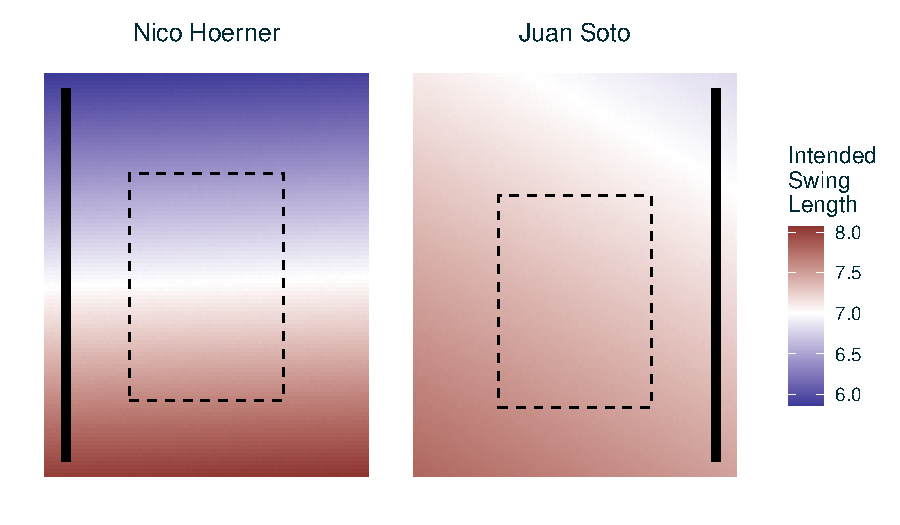
\includegraphics[width = 0.8\textwidth]{../../figures/adaptation.pdf}
        \caption{\it Expected swing length by pitch location for two sample batters: Nico Hoerner (left) and Juan Soto (right), from the perspective of behind home plate. The thick vertical bars show the side of the plate on which the batter stands, and the dashed rectangle shows the strike zone, which depends on the height and stance of the batter. The color shows the predicted swing length  from model (\ref{eqn:intention-swing-length}) assuming a 0-0 count.}
        \label{fig:adaptation}
      \end{figure}


      \begin{figure}
        \centering
        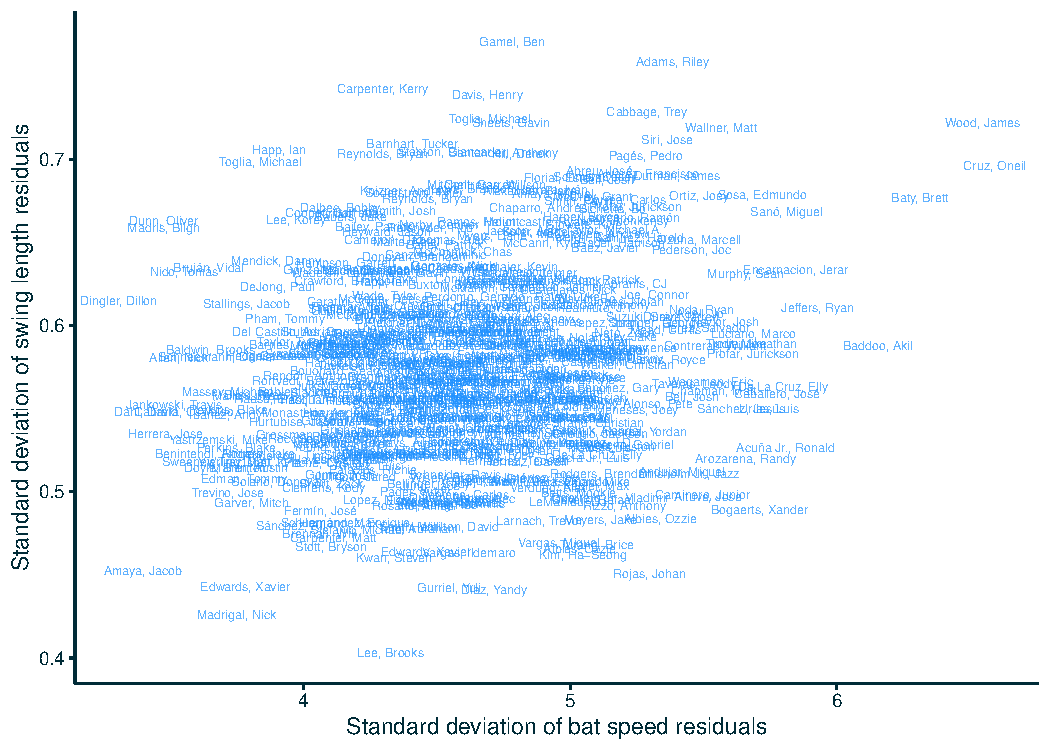
\includegraphics[width = 0.8\textwidth]{../../figures/residual_sd.pdf}
        \caption{\it Insert meaningful caption here...}
        \label{fig:resid-sd}
      \end{figure}

  \section{Discussion}
  \label{sec:discussion}

    \subsection{Future Work}
    \label{sec:future-work}

      \begin{itemize}
        \item batter-specific approach values (as opposed to applying approach to average batter)
        \item valuing tradeoffs considering base-out situation (e.g. runner on third, less than two outs)
        \item future data coming down the pipeline from MLBAM
      \end{itemize}

  % This nastiness for the bibliography to work both locally and on Overleaf
  % https://tex.stackexchange.com/questions/623701/path-for-bib-file-working-simultaneously-in-texstudio-and-overleaf
  \bibliography{\ifnum\pdfstrcmp{\jobname}{output}=0 reports/swingfastslow\else ../swingfastslow\fi}

\end{document}